\documentclass{report}
\usepackage[utf8]{inputenc}
\usepackage[spanish]{babel}
\usepackage[letterpaper, portrait, margin=2cm]{geometry}
\usepackage[style=ieee]{biblatex}
\usepackage{amsthm}
\usepackage{amsmath}
\usepackage{amssymb}
\usepackage{amsfonts}
\usepackage{hyperref}
\usepackage{csquotes}
\usepackage{mathtools}
\usepackage{graphicx}
\usepackage{float}
\usepackage{array}

\addbibresource{bibliography.bib}

\newtheorem{definition}{Definición}

\DeclarePairedDelimiter{\ceil}{\lceil}{\rceil}

\title{Anteproyecto de Investigación: Modelo de muestreo virtual de suelos agrícolas para analítica en base al muestreo aleatorio simple y estratificado}
\author{Tobias Briones}
\date{Septiembre 2021}


\begin{document}

\makeatletter
    \begin{titlepage}
        \begin{center}
            
\includegraphics[width=0.3\linewidth]{ref/logo-unah.png}\\[4ex]
            {\huge \bfseries \@title 
            \vspace{1cm}}\\[2ex]
            {\LARGE \@author}\\[50ex] 
            
            {\large
            Anteproyecto de seminario de investigación presentado a la\\
            Universidad Nacional Autónoma de Honduras de la carrera de\\
            Licenciatura en Matemática
            }\\[2ex]
            
            {\large \@date}
        \end{center}
    \end{titlepage}
\makeatother
\thispagestyle{empty}
\newpage

\thispagestyle{empty}
\tableofcontents
\listoffigures
\newpage

\chapter{Introducción}

En la ciencia de datos se hacen procesos complicados para obtener valor a partir de los datos crudos de los usuarios de forma que se puedan entrenar modelos para hacer predicciones, prescripciones e investigación de los problemas de las empresas en base a caso por caso. Uno de los primeros pasos en el proceso consiste en obtener datos existentes y que sufran una transformación para que se filtren o curen y por tanto se obtengan datos relevantes al estudio. Así como determinar la clasificación correcta de los datos, determinar variables de estudio, desnormalizar bases de datos, encontrar patrones y establecer  interpretaciones \cite{university-of-wisconsin-data-science-2021}. Debido a estos retos técnicos, el analista de datos debe de contar como entrada con todos los datos e historiales de la empresa que se va a analizar en ese dominio.

\bigbreak

A fin de obtener los datos de fincas, granjas o terreno agrícola es requerido muchas veces realizar muestreo de suelo. Algunos de los casos de uso son diagnóstico de fertilidad \cite{lassaga-2011} y análisis de contaminantes \cite{gobpe-ministerio-del-ambiente-2014}. Es determinante construir resultados a partir de estos datos para dar resultados en base a zafra y sus correspondiente diagnóstico de optimalidad.

\bigbreak

Existen varios enfoques de muestreo de una población, la mayor parte de las veces se basan en un muestreo aleatorio simple. Para poder diseñar un muestreo para un caso en particular es requerido llevar a cabo encuestas puntuales al personal del área agrícola a fin de conocer el terreno y sus clasificaciones \cite{organizacion-de-las-naciones-unidas-para-la-agricultura-y-la-alimentacion-1990}.

\section{Justificación}

El propósito de esta investigación es diseñar una metodología eficiente que permita modelar los suelos agrícolas de forma que se puedan obtener muestras representativas de estos y posteriormente ser utilizables para que permitan desarrollar proyectos con el sector agrícola integrando los resultados obtenidos de esta investigación. Se ha propuesto como objetivo emprender una investigación en este campo relacionado con el análisis de los suelos agrícolas para poder eventualmente publicar los resultados e integrar los modelos obtenidos en proyectos de analítica. Esto se espera que permita a las empresas de analítica poder proveer servicios/productos con un estado del arte en la región para sus prospectos clientes los cuales consisten en empresas agrícolas que deberían automatizar y llevar a cabo el análisis de suelos de forma más moderna que como lo hacen actualmente o, en el peor de los casos, no hacen ni son capaces de entender ningún análisis ni optimización u automatización en absoluto. Los beneficiados serán empresas del sector agrícola en Honduras al poder modelar sus suelos o lotes y así optimizar sus operaciones mediante técnicas de análisis de datos. Los recursos para realizar la extracción de datos en el suelo agrícola son muy limitados ya que la población es demasiado grande. Se debe poder entrenar los respectivos modelos de analítica a partir de los datos obtenidos del muestreo el cual debe ser suficientemente representativo y pequeño para poder llevar a cabo esta extracción de datos utilizando los recursos limitados que se tienen disponibles.

\bigbreak

Como limitantes en este proyecto se encuentran: la cota de tiempo para su realización consistente en un curso trimestral de seminario de investigación; llevar a cabo la recopilación física de datos o muestras. Debido a estas limitaciones se define el alcance del proyecto abajo.

\section{Alcance}

Dado las limitantes de esta investigación, se procederá a realizar las siguientes metas:

\begin{itemize}
    \item Obtener los modelos iniciales ya establecidos.
    
    \item Crear modelos ad hoc parar introducir definiciones de negocio. Esto con visión a que estos resultados deben de poder utilizarse en pro para software de analítica.
    
    \item Desarrollar gráficos, herramientas o simulaciones necesarias para la explicación de los fenómenos. En caso de requerir programación, se utilizará Python ya que se tratan de prototipos y se acopla perfectamente a este proyecto de investigación.
    
    \item Crear entrevistas/encuestas con personal del sector agrícola en caso de requerirlo.
\end{itemize}

\bigbreak

\chapter{Planteamiento del problema}

\section{Hipótesis}

Todos los suelos agrícolas se pueden particionar como lotes y existe una relación de homogeneidad entre cada lote.

\section{Objetivos}


\subsection{Objetivo general}

Demostrar un proceso en el cual se pueda crear muestras representativas de lotes de zona agrícola tal que sean eficientes tanto de extraer como de obtener resultados de analítica a partir de ellas.

\subsection{Objetivos específicos}

\begin{itemize}
    \item Encontrar inductivamente modelos generales para analizar los suelos y lotes. 
    \item Diseñar un proceso para determinar un muestreo estratificado de lotes.
    \item Establecer un marco teórico estadístico para medir las variables en cuestión.
    \item Diseñar un modelo de selección de lotes por homogeneidad.
    \item Medir las relaciones para determinar cuan fina sera la partición.
    \item Concluir en un resultado final que pueda ser utilizado por software de analítica.
\end{itemize}


\section{Preguntas de investigación}


\section{Metodología}


\chapter{Marco teórico}

Entre los tipos de muestreo que se han encontrado útiles para medir los suelos agrícolas se tienen:

\begin{itemize}
    \item \textbf{Muestreo Aleatorio Simple MAS:} Consiste en tomar $n$ puntos aleatorios de la población. Estos puntos deben de tener la misma probabilidad de ser escogidos para que la muestra sea representativa y se toman de forma "mezclada". Por ejemplo, la sangre esta "mezclada" en el cuerpo humano, por lo que al tomar una muestra de solo una pizca basta para hacer los análisis ya que esa pizca obtenida es igual que todas las demás.
    
    \item \textbf{Muestreo Simple Estratificado:} Esta es una técnica de muestreo que será muy útil en el modelado de los suelos agrícolas. La población se particiona en subconjuntos de diferentes tipos y homogéneos de forma que se puede realizar un MAS en cada subconjunto homogéneo de la partición. Por ejemplo, los lotes se pueden particionar como: área forestal, con problemas, bosque, construcción, etc.
    
    \item \textbf{Muestreo sistemático:} En este muestreo se toma un punto aleatorio y se mide por cada $n$-ésima unidad de forma que se lleva un espaciado constante a partir del punto inicial. Por ejemplo, este tipo de muestreo es utilizado para medir el suelo cuando es rectangular a lo largo de su perímetro o también cuando es de forma irregular.
\end{itemize}

\subsection{Marco para muestreo}

El marco para muestreo \cite{lohr-2009} consiste en definir el espacio de la población (el universo) de donde se obtendrán las posibles muestras (subconjuntos) y estas muestras contienen las unidades que serán seleccionadas. Se nota que cada muestra tiene una probabilidad de ser escogida y para cada muestra, cada unidad tiene también una probabilidad para ser escogida.

\begin{definition}[Universo]
    El \textbf{Universo} o \textbf{Población finita} de $N$ unidades es el conjunto índice
    $$
    U = \{ 1, 2, ..., N \}
    $$
    Donde $N \in \mathbb{N}$ es el tamaño de la población.
\end{definition}

\begin{definition}[Muestra]
    Sea $U$ el conjunto universo. Un conjunto $S$ es una muestra para $U$ si $S \subseteq U$.
\end{definition}

\begin{definition}[Probabilidad de una muestra]
    Si $S$ es una muestra. $S$ tiene una probabilidad de ser escogida de $P(S)$.
\end{definition}

Notar que la probabilidad de todas las muestras de ser escogida es $1$. Esto es, $\forall S_i \in D \implies \sum_{i=1}^{N} P(S_i) = 1$, donde el conjunto $D$ es el diseño escogido, esto es, una colección de subconjuntos (muestras) de $U$.

\bigbreak

Según las definiciones de arriba, cada muestra $S_i$ tiene probabilidad $P(S_i)$ de ser seleccionada. Ahora, cada unidad tiene una probabilidad de terminar siendo seleccionada si pertenece a una de las muestras que se seleccionó.

\begin{definition}[Probabilidad de una Unidad]
    La probabilidad de que una unidad $x$ sea seleccionada en una colección de muestras $D = \{ S_1, S_2, ..., S_n \}$ se define como
    
    $$
    \pi_x = P(\text{unidad $x$ está en la muestra}) = \sum_{S_i \in \{ S \in D | x \in S \}} P(S_i)
    $$
\end{definition}

Es decir, para calcular la probabilidad de que la unidad $x$ sea seleccionada, se hace la suma de las probabilidades de todas las muestras que contienen a $x$.

Con respecto a los intervalos de confianza, se deberá repetir muchas veces el muestreo para por determinar su confianza. Son útiles en el caso no-ideal donde no se conoce toda la población. Los intervalos de confianza se construyen como \cite{the-pennsylvania-state-university-no-date}:

\begin{definition}[Intervalo de confianza]
    Un \textbf{intervalo de confianza} es un rango que se calcula usando estadística para estimar un parámetro desconocido de la población con un nivel determinado de confianza. 
\end{definition}

\begin{definition}[Estimación puntual]
    La \textbf{estimación puntual} es una muestra estadística que sirve como los mejores estimados para un parámetro de la población.
\end{definition}

\begin{definition}[Margen de error]
    El \textbf{margen de error} de un intervalo de confianza es la mitad de su ancho.
\end{definition}

\subsection{Estimar el tamaño de la muestra}

Al estimar el tamaño de la muestra se tiene en cuenta otras definiciones como el margen de error que se considera tolerable. Las encuestas se pueden llevar a cabo para obtener estas condiciones correctamente. Para obtener resultados con respecto al tamaño de muestra preferible se sugiere \cite{lohr-2009}:

\begin{enumerate}
    \item Preguntárse: ¿Qué se espera de la muestra, y cuánta precisión se necesita?, ¿Qué consecuencias tienen los resultados del muestreo?, ¿Cuánto error es tolerable?.
    
    \item Encontrar una ecuación que relacione el tamaño de la muestra $n$ y las expectativas de la muestra.
    
    \item Estimar cualquier cantidad desconocida y resolver para $n$.
    
    \item Iterar estos pasos para obtener mejores valores de acuerdo a las expectativas. Si ni siquiera hay recursos disponibles para este proceso, entonces la investigación no se podrá llevar a cabo.
\end{enumerate}

\subsection{Muestreo aleatorio simple (MAS)}

Este tipo de muestreo es el más básico que se puede tomar y en base a él se desarrollan en gran medida los otros tipos de muestreo más compuestos. Las condiciones para que funciones son que las unidades de la población tenga igual probabilidad de ser escogidas. Los cálculos hechos para el MAS son también extendidos por otros métodos de muestreo, ya que al final siempre conllevan con algo de aleatoriedad. 

\bigbreak

Es importante que el suelo sea homogéneo para realizar un muestreo simple aleatorio y probablemente también mezclar las muestras para obtener un compuesto. Para realizar el muestreo se pueden seguir varios patrones, a saber, zigzag, diagonal, etc.:

\begin{figure}[H]
    \centering
    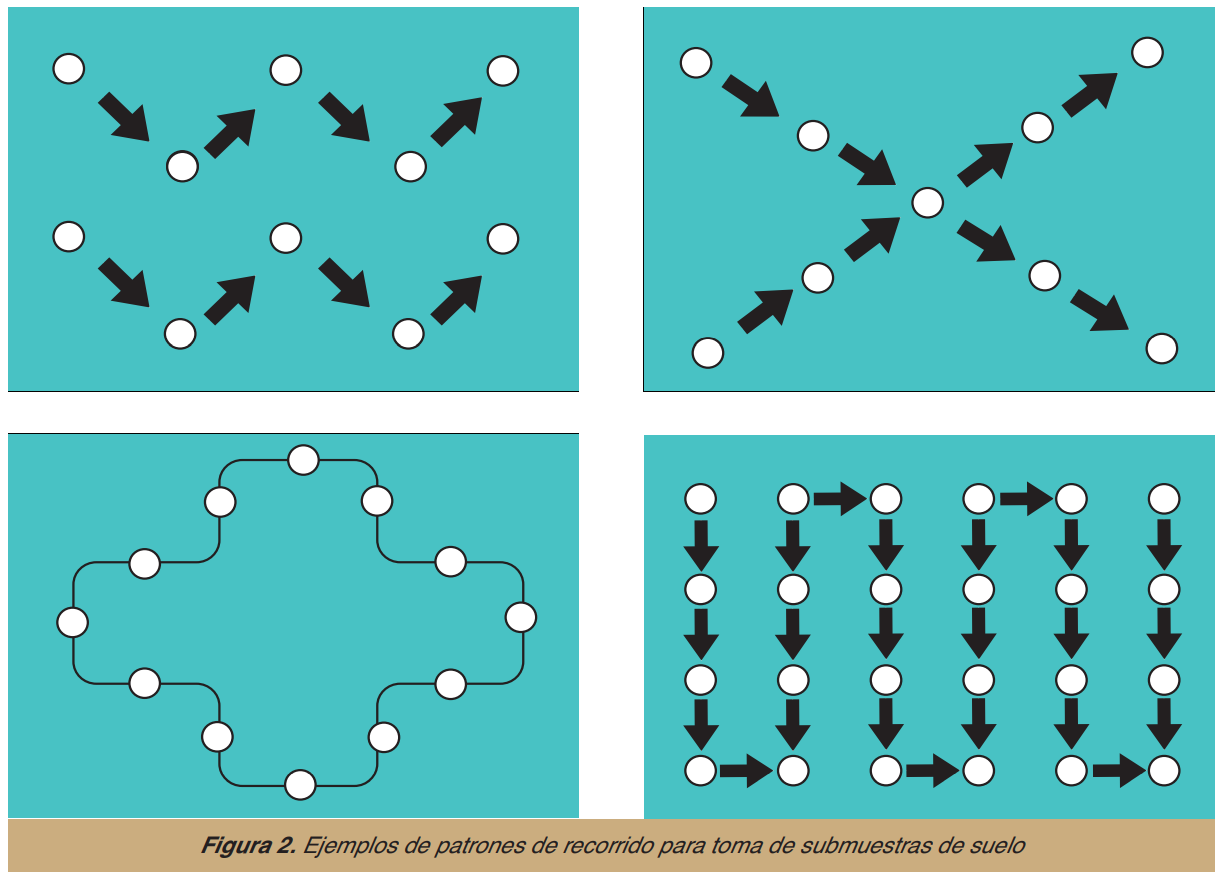
\includegraphics[width=0.3\paperwidth]{ref/sampling-patterns-srs.png}
    \caption{Patrones de muestreo para análisis de fertilidad de suelo \cite{lassaga-2011}}
\end{figure}

Como se detalla más adelante, el terreno o lotes también se puede estratificar y realizar un MAS en cada estrato obtenido. El muestro sistemático por otra parte puede llegar a reducirse a un MAS o similar dado las condiciones apropiadas. Esto indica que el MAS es elemental para hacer otro tipo de diseño de muestreo.

\bigbreak

Estas son los resultados para los cálculos del MAS \cite{thompson-2012}:

\bigbreak
\textbf{Media de la población}

\bigbreak

$\overline{x}_U = \frac{1}{N}(x_1 + x_2 + ... + x_N) = \frac{1}{N} \sum_{i=1}^N x_i$


\bigbreak
\textbf{Media de la muestra}

\bigbreak

$\overline{x} = \frac{1}{n}(x_1 + x_2 + ... + x_N) = \frac{1}{n} \sum_{i=1}^n x_i$


\bigbreak
\textbf{Varianza de la población finita} En MAS, la varianza de la muestra $s^2$ es una estimación no-alineada de la varianza para la población finita

\bigbreak

$\sigma ^2 = \frac{1}{N-1} \sum_{i=1}^{N} (x_i - \overline{x}_U)^2$


\bigbreak
\textbf{Varianza de la muestra}

\bigbreak

$s^2 = \frac{1}{n-1} \sum_{i=1}^n (x_i - \overline{x}_U)^2$


\bigbreak
\textbf{Total de la población}

\bigbreak

$t = \sum_{i=1}^N x_i = N \overline{x}_U$


\subsection{Muestreo sistemático}

Para realizar un muestreo sistemático se siguen los siguientes cálculos:

\bigbreak

Dado el tamaño de la población $N$ y el número de muestras $n$, hacer $k=\ceil{\frac{N}{n}}$. El valor $k$ es el período que hace que el muestreo sea sistemático. Tomar un punto aleatorio $K \in [1, k]$. Cada unidad dada por $K$, $K + k$, $K + 2k$, ... , etc., define la muestra.

\bigbreak

En ciertos casos el muestreo sistemático es el mismo MAS por lo que se pueden aplicar técnicas del MAS. Otras veces funciona como un intermediario (proxy) hacia el MAS ya que como se puede notar, si la población está dispuesta de forma aleatoria entonces lo que se tendría sería básicamente un MAS. También se debe tener en cuenta que la probabilidad de un grupo de ser escogido no es la misma como en el MAS. Otro uso que puede tener este tipo de muestreo es de hacer un trabajo similar al muestreo por clúster. De estos factores depende que la muestra sea representativa ya que si la población está ordenada de acuerdo a su índice entonces la muestra no servirá (p. ej. solo salen unidades del mismo tipo al estar ordenadas por posición, si hay hombres y mujeres solo salen hombres por ser posición par). 

\bigbreak

\begin{figure}[H]
    \centering
    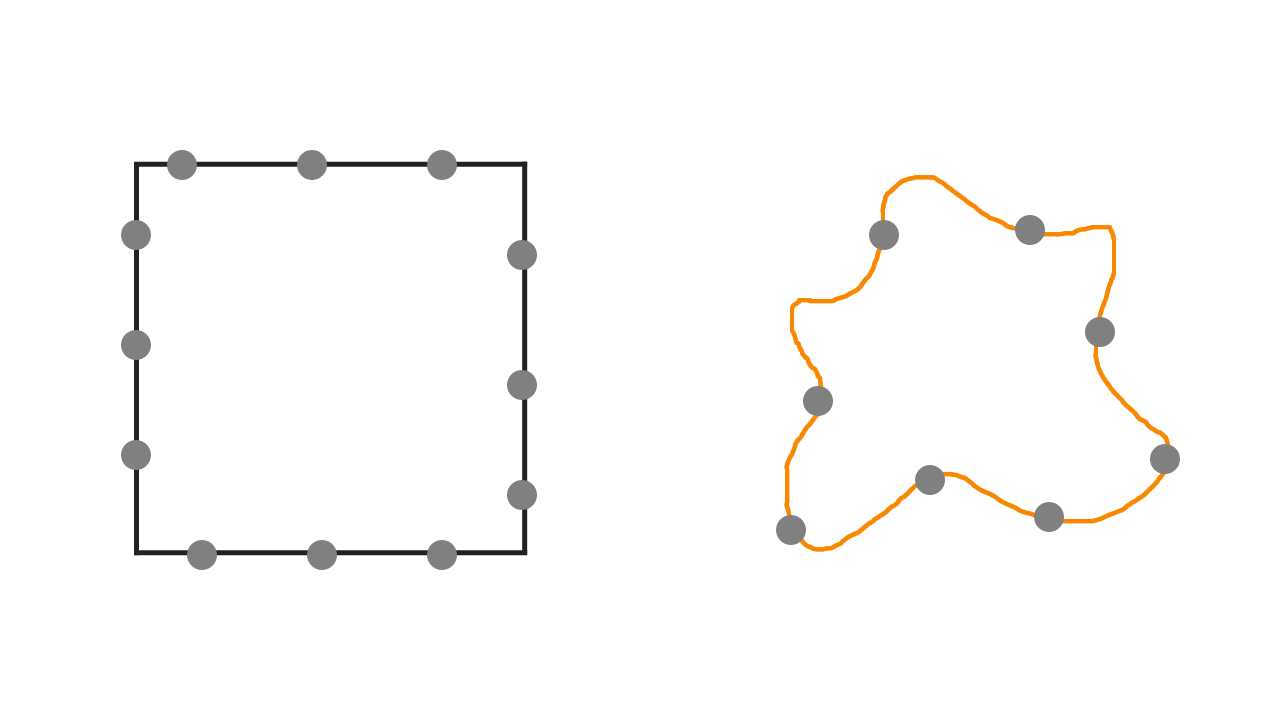
\includegraphics[width=0.3\paperwidth]{img/soil-systematic-sampling.png}
    \caption{Posible muestreo sistemático de un lote}
\end{figure}

La ilustración de arriba describe una de muchas estrategias \cite{lassaga-2011} \cite{gobpe-ministerio-del-ambiente-2014} para tomar las muestras del suelo. En este caso se toma el perímetro del suelo y sistemáticamente se toman las muestras por el perímetro, las cuales también pueden ser determinadas por otros patrones como diagonal o zigzag.

\bigbreak

Hay que tomar en cuenta que el muestreo sistemático no siempre produce una muestra representativa por lo dicho más arriba, esto es, cuando hay una distribución periódica de las unidades. Para los estudios ecológicos de suelos \cite{lohr-2009}: "Puede haber una topografía de crestas y surcos que daría lugar a un patrón periódico de vegetación. Si un esquema de muestreo sistemático sigue el mismo ciclo, la muestra no se comportará como una MAS".

\subsection{Muestreo estratificado}

Como se ha mencionado, este es uno de los temas centrales de esta investigación ya que los suelos agrícolas se pueden \textit{particionar} en lotes los cuales tienen atributos que permiten su medición y se espera poder llegar a establecerlos como homogéneos para poder elaborar el diseño del muestreo correspondiente.

\bigbreak

La población se debe de dividir (particionar) en \textbf{estratos} que sean disjuntos a dos. Esto viene de la clásica estratificación por capas. Así, para una población de tamaño $N$, se divide en $H$ estratos o capas con $N_h$ unidades en el estrato $H$. Es necesario conocer $N_1$, $N_2$, ... , $N_H$ y por tanto se tiene que $N_1 + N_2 + \cdot \cdot \cdot + N_H = N$.

\bigbreak

Para hacer un \textbf{muestreo estratificado aleatorio} como es de esperar, se toma cada estrato de $N_h$ unidades y se hacen $n_h$ mediciones aleatorias ($n_h < N_h$). Entonces el tamaño de la población se encuentra dado por $n = \sum_{i=1}^H n_i$.

\bigbreak

\begin{figure}[H]
    \centering
    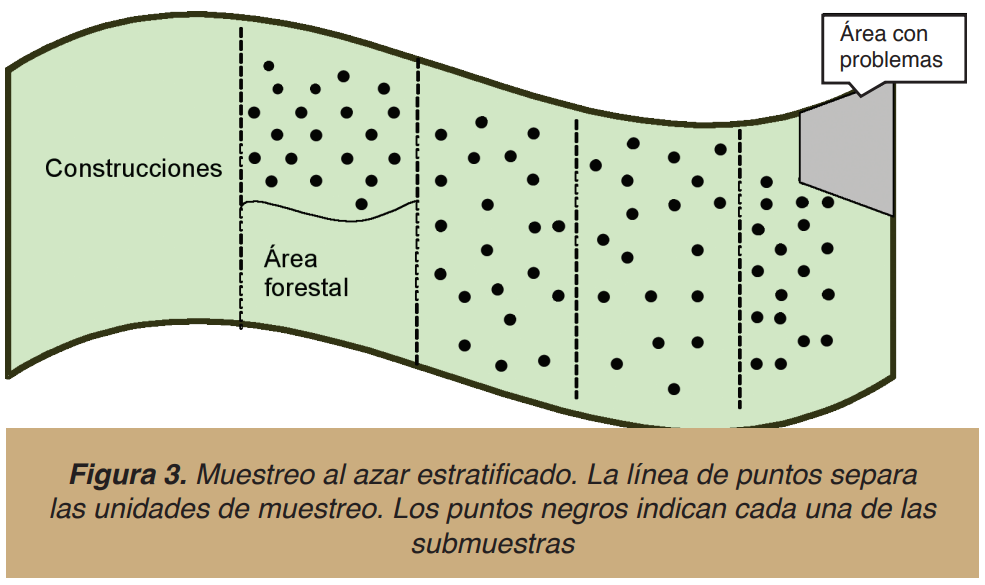
\includegraphics[width=0.5\paperwidth]{ref/stratified-sampling-examples.png}
    \caption{Ejemplo de estratos para diagnóstico de fertilidad \cite{lassaga-2011}}
\end{figure}

Como resumen de los tipos de muestreos de utilidad se puede ilustrar el siguiente ejemplo:

\begin{figure}[H]
    \centering
    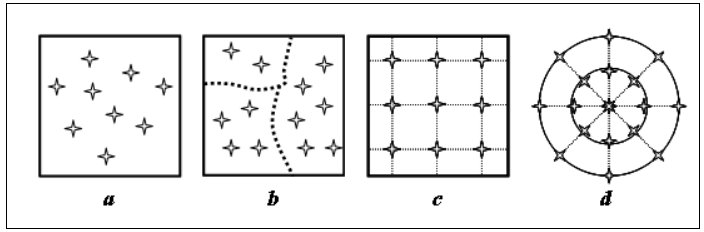
\includegraphics[width=0.5\paperwidth]{ref/kind-of-samplings-example.png}
    \caption{Ejemplo de tipos de muestreos. a) aleatorio simple, b) aleatorio estratificado, c) sistemático rejilla rectangular, d) sistemático rejilla polar \cite{unknown-author-2007}}
\end{figure}

Sea $S_h$ el conjunto de $n_h$ unidades para el estrato $h$. El valor de la unidad \textit{jth} en el estrato $h$ se define como $x_{hj}$. Se siguen las siguientes valoraciones para el muestreo estratificado \cite{lohr-2009}:

\bigbreak

\textbf{Población total en el estrato H}
\bigbreak
$t_h = \sum_{j=1}^{N_h} x_{hj}$


\bigbreak

\textbf{Total de la población}
\bigbreak
$t = \sum_{h=1}^H t_h$


\bigbreak

\textbf{Media de la población para el estrato $h$}
\bigbreak
$\overline{x}_{hU} = \frac{\sum_{j=1}^{N_h} x_{hj}}{N_h} = \frac{t_h}{N_h}$


\bigbreak

\textbf{Media de la población en general}
\bigbreak
$\overline{x}_U = \frac{\sum_{h=1}^H \sum_{j=1}^{N_h} x_{hj}}{N} = \frac{t}{N}$


\bigbreak

\textbf{Varianza de la población en el estrato $h$}
\bigbreak
$S_h^2 = \sum_{j=1}^{N_h} \frac{(x_{hj} - \overline{x}_{hU})^2}{N_h - 1}$


\bigbreak

A partir de aquí, otros cálculos para los MAS se pueden aplicar para cada estrato. Se tiene que:

\bigbreak

$\overline{x}_h = \frac{1}{n_h} \sum_{j \in S_h} x_{hj}$

\bigbreak

$s^2_h = \sum_{j \in S_h} \frac{(x_{hj} - \overline{x}_h)^2}{n_h - 1}$

\subsection{Encuestas agrícolas}

A fin de obtener información precisa para poder diseñar un muestreo representativo y eficiente puede ser necesario hacer un análisis mediante encuestas y poder obtener uno de los modelos de muestreo que se conocen.

\bigbreak

Las encuestas agrícolas son muy complicadas y tienen un gran número de variables las cuales pueden comprender en tanto de \cite{organizacion-de-las-naciones-unidas-para-la-agricultura-y-la-alimentacion-1990}:

\begin{itemize}
    \item Herramientas, maquinarias, fertilizantes, plaguicidas, semillas y otros insumos.
    \item Superficie total y régimen de tenencia.
    \item Superficie bajo cultivos y producción.
    \item Verduras, frutas, nueces.
    \item Ganadería, avicultura, estabulación.
    
    \item Pesca, caza y explotación maderera.
    \item Regadío, pozos, avenamiento y cercado.
    \item Ingresos, comercialización, gastos, ahorros.
    \item Recuento y características de la población; mano de obra no pagada.
    \item Sanidad, educación, ocupación y estadísticas sociales de la población agrícola.
    \item Hogares y edificios agrícolas.
    \item Transporte y comunicaciones de la población agrícola.
    \item Fuentes y consumo de alimentos.
    \item Encuestas de opinión acerca de las políticas, métodos, productos, etc.
\end{itemize}

\bigbreak
    
Además de utilizar estas variables, se puede obtener más datos a partir de variables auxiliares. Con respecto a las fuentes de datos se puede acceder a los productores y las operaciones agrícolas, hogares agrícolas en relación con otros datos.

\bigbreak

Las encuestas agrícolas suelen ser muy variadas, cada variable que se ha enumerado tiene sus propias variaciones y propósitos múltiples. Por esto observamos que se deberá recurrir a \textbf{encuestas multitemáticas}. Además, también se necesitan aplicar métodos múltiples ya que las mediciones que se hacen requieren métodos diferentes de medición.
    
\section{Anexos}

Se ha tomado nota en pequeña parte sobre la elaboración y estructura de \textit{Manual de Elaboración y Presentación de Tesis} \cite{universidad-san-carlos-2016}, \textit{Metodología de la investigación} \cite{collado-2014}, \textit{Introducción a la metodología de la investigación científica} \cite{cabezas-2018} para esta propuesta de investigación.

\printbibliography

\end{document}
